\chapter{Background}

\section{The Finite Element Method}
\label{sec:bkg:fem}
Computational methods based upon finite elements are used to approximate the solution of partial differential equations (henceforth, PDEs) in a wide variety of domains. The mathematical abstraction used in finite element methods (or FEMs) is extremely powerful: not only does it help reasoning about the problem, but also provides systematic ways of deriving effective computer implementations. In~\cite{brenner-and-scott}, it is usefully suggested to consider an FEM as a black box that, given a differential equation, returns a discrete algorithm capable of approximating the equation solution. Unveiling the whole magic of such a black box is clearly out of the scope of this chapter. We rather limit ourselves to review the mathematical properties and the computational aspects that are essential for understanding the contributions in Chapters~\ref{ch:optimality} and~\ref{ch:lowlevelopt}. The content and the notation used in this section are inspired by~\cite{florian-thesis},~\cite{Fenics} and~\cite{quadrature-olegaard}. For a complete treatment of the subject, the reader is invited to refer to~\cite{brenner-and-scott}.



\subsection{Variational Formulation}
\label{sec:bkg:var-problems}
We consider the weak formulation of a {\em linear variational problem}

\begin{equation}
\begin{split}
\text{Find}\ u \in U\ \text{such that} \\
a(u, v) = L(v), \forall v \in V
\end{split}
\end{equation}

where $a$ and $L$ are, respectively, a bilinear form and a linear form. The term ``variational'' stems from the fact that the function $v$ can vary arbitrarily. The unfamiliar reader may find this expression unusual. Understanding the actual meaning of this formulation is far beyond the goals of this review, since an entire course in functional analysis would be needed. Informally, we can think of $V$ as a ``very nice'' space, in which functions have desirable properties. The underlying idea of the variational formulation is to ``transfer'' certain requirements (e.g., differentiability) from the unknown $u \in U$ to $v \in V$.

The sets $U$ and $V$ and called, respectively, trial and test functions. The variational problem is discretized by using discrete test and trial spaces

\begin{equation}
\label{sec:bkg:eq:disc-var}
\begin{split}
\text{Find}\ u_h \in U_h \subset U\ \text{such that} \\
a(u_h, v_h) = L(v_h), \forall v_h \in V_h \subset V
\end{split}
\end{equation}

Let $\lbrace \psi_i \rbrace_{i=1}^N$ be the set of basis functions spanning $U_h$ and let $\lbrace \phi_j \rbrace_{j=1}^{N}$ be the set of basis functions spanning $V_h$. Then the unknown solution $u$ can be approximated as a linear combination of the basis functions $\lbrace \psi_i \rbrace_{i=1}^N$,

\begin{equation}
u_h = \sum_{j=1}^N U_j \psi_j.
\end{equation}

This allows us to rewrite~\ref{sec:bkg:eq:disc-var} as:

\begin{equation}
\sum_{j=1}^N U_j a(\psi_j, \phi_i) = L(\phi_i),\ i=1,2,...,N
\end{equation}

From the solution of the following linear system we determine the set of {\em degrees of freedom} $U$ to express $u_h$:

\begin{equation}
\label{sec:bkg:eq:lin-sys}
Au = b
\end{equation}

where clearly

\begin{equation}
\label{sec:bkg:eq:disc-op}
\centering
\begin{split}
A_{ij} = a(\phi_i(x), \phi_j(x)) \\
b_i = L(\phi_i(x))
\end{split}
\end{equation}

The matrix $A$ and the vector $b$ can be seen as the discrete operators arising from the bilinear form $a$ and from the linear form $L$ for the given choice of basis functions.

The variational formulation of a {\em non-linear variational problem} requires refinements that are out of the scope of this review. The interested reader is again invited to refer to~\cite{brenner-and-scott}.

\subsection{Finite Elements}
In an FEM the domain $\Omega$ of the PDE is partitioned into a finite set of disjoint cells $\lbrace K \rbrace$; that is, $\bigcup K = \Omega$ and $\bigcap K = \emptyset$. This forms a {\em mesh}. Formally, A finite element is a triple ${<}K,\mathcal{P}_K,\mathcal{L}_K{>}$, where:
\begin{itemize}
\item $K$ is a cell in the mesh with non-empty interior and piecewise smooth boundary;
\item $\mathcal{P}_K$ is a finite dimensional ``local'' function space of dimension $n_K$;
\item the set of degrees of freedom $\mathcal{L}_K$ is a basis $\lbrace l_1^K, l_2^K, ..., l_{n_K}^K\rbrace$ for $\mathcal{P}'_K$, the dual space of $\mathcal{P}_K$. 
\end{itemize}
This definition allows to impose constraints on the set of basis functions $\lbrace \phi_1^K, \phi_2^K, ..., \phi_{n_K}^K\rbrace$ spanning $\mathcal{P}_K$. For instance, to enforce a {\em nodal basis} for $\mathcal{P}_K$ -- a particularly useful property for expressing solutions in $U_h$ -- we can impose that the relationship

\begin{equation}
l_i^K(\phi_j^K) = \delta_{ij},\ i,j = 1,2,...,n_K
\end{equation}

must be satisfied ($\delta_{ij}$ is the Kronecker delta). This allows to express any $v \in \mathcal{P}_K$ as

\begin{equation}
v = \sum_{i=1}^{n_K} l_i^K(v) \phi_i^K.
\end{equation}

Each linear functional in $\mathcal{L}_K$ is used to evaluate one degree of freedom of $v$ in terms of the chosen nodal basis. In other words, we can refer to both the coefficients $U$ introduced in the previous section and $\mathcal{L}_K$ as the degrees of freedom.

\paragraph{Example: the triangular Lagrange element}
The following example is extracted from~\cite{Fenics}. Consider a triangular cell $K$ and let $\mathcal{P}_K$ be the space of polynomials of order $1$ on $K$. $\mathcal{L}_K$ may be the set of bounded linear functionals representing point evaluation at the vertices $\boldsymbol{x}^i$ ($i=1,2,3$) of $K$ such that

\begin{equation}
\centering
\begin{split}
l_i^K : \mathcal{P^K} \rightarrow \mathbb{R} \\
l_i^K(v) = v(\boldsymbol{x}^i)
\end{split}
\end{equation}

Since if $v$ is zero at each vertex then $v$ must be zero everywhere, $\mathcal{L}_K$ really is a basis for $\mathcal{P}'_K$, so what we have defined is indeed a finite element. In particular, if we take $\boldsymbol{x}^1 = (0, 0),\ \boldsymbol{x}^2 = (1,0),\ \boldsymbol{x}^3 = (0,1)$, we have that the nodal basis is given by:

\begin{equation}
\phi_1(\boldsymbol{x}) = 1 - x_1 - x_2,\ \ \phi_2(\boldsymbol{x}) = x_1,\ \ \phi_3(\boldsymbol{x}) = x_2.
\end{equation}


\subsection{Global Discretization}
\label{sec:bkg:refel}
A {\em local-to-global mapping} allows to patch together the finite elements to form a global function space, for instance the set of trial functions $U_h = \operatorname{span}\lbrace \psi_i \rbrace_{i=1}^N$ introduced in Section~\ref{sec:bkg:var-problems}. A local-to-global mapping is a function

\begin{equation}
\iota_K : [1,n_K] \rightarrow [1,N]
\end{equation}

that maps the local degrees of freedom $\mathcal{L}_K$ to global degrees of freedom $\mathcal{L}$. The mappings $\iota_K$, together with the choice of $\mathcal{L}_K$, determine the continuity of a function space or, in simpler words, the continuity of a function throughout the domain $\Omega$. The reader is invited to refer to~\cite{Fenics} for a comprehensive description of this step.

One of the crucial aspects of an FEM is that global function spaces are often defined in terms of a {\em reference finite element} ${<}\hat{K}, \hat{\mathcal{P}}, \hat{\mathcal{L}}{>}$ and a set of invertible mappings $\lbrace \mathcal{G}_K\rbrace_{K}$ from $\hat{K}$ to each cell in the mesh such that $K = \mathcal{G}_K(\hat{K})$.  This situation is illustrated in Figure~\ref{fig:bkg:reference-el}.

\begin{figure}
\begin{CenteredBox}
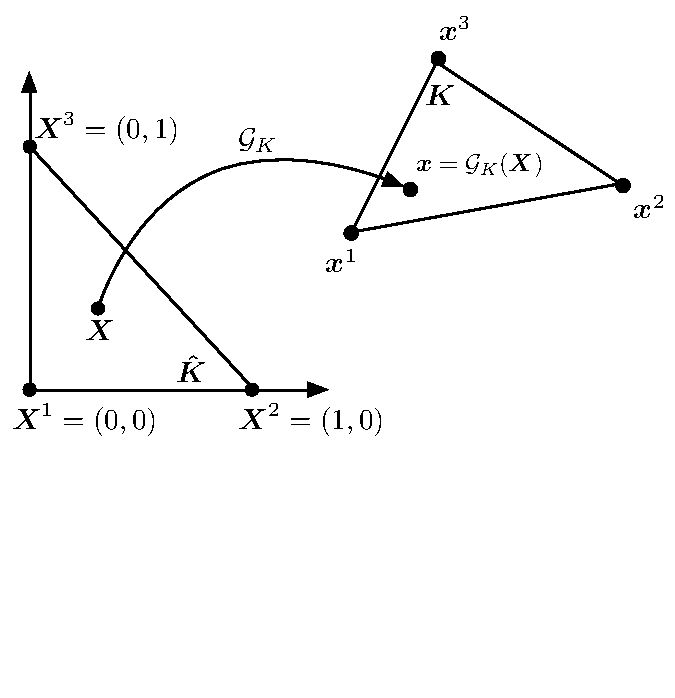
\includegraphics[scale=0.8]{background/figures/reference-element}
\end{CenteredBox}
\caption{Affine mapping from the reference element $\hat{K}$ to an element $K$.}
\label{fig:bkg:reference-el}
\end{figure}

For each $K$, $\mathcal{G}_K$ also allows to generate $\mathcal{P}_K$ and $\mathcal{L}_K$.  The complexity of this process depends on the mapping itself. In the simplest case, the mapping is affine; that is, expressible as $\mathcal{G}_K(\hat{\boldsymbol{x}}) = A_K \hat{\boldsymbol{x}} + b_K$, where $A_K$ and $b_K$ are, respectively, some matrix and vector.


\subsection{Assembly}
\label{sec:bkg:assembly}
The {\em assembly} of an FEM is the phase in which the matrix $A$ and the vector $b$ from~\ref{sec:bkg:eq:disc-op} are constructed. This is accomplished by adding the contributions from each $K$ to $A$ and $b$. Let us consider the bilinear form $a$, and assume this is an integral over $\Omega$. Thanks to the linearity of the operator, we can express $a$ as

\begin{equation}
a = \sum_{K} a_K
\end{equation}

where $a_K$ is an element bilinear form. We can then define the local element matrix

\begin{equation}
A_i^K = a_K (\psi_{i_1}^K, \phi_{i_2}^K)
\end{equation}

where $i \in \mathcal{I}_K$ is the index set on $A_i^K$. That is, $\mathcal{I}_K = \lbrace (1,1), ..., (n_U, n_V) \rbrace$, with $n_U$ and $n_V$ representing the number of degrees of freedom for the local trial functions $\psi^K \in U_h^K$ and the local test functions $\phi^K \in V_h^K$. The element matrix $A^K$ is therefore a (typically dense) matrix of dimension $n_U \times n_V$.

Now let $\iota_K^U$ and $\iota_K^V$ be the local-to-global mappings for the local discrete function spaces $U_h^K$ and $V_h^K$. We can define, for each $K$, the collective local-to-global mapping $\iota_K : \mathcal{I}_K \rightarrow \mathcal{I}$ such that

\begin{equation}
\iota_K (i) = (\iota_K^U(i_1), \iota_K^V(i_2))\ \forall i \in \mathcal{I}_K.
\end{equation}

This simply maps a pair of local degrees of freedom to a pair of global degrees of freedom. Let also $\mathcal{T}$ be the subset of the cells in the mesh in which $\psi_{i_1}$ and $\phi_{i_2}$ are both non-zero. Note that here we are talking about the global functions whose restrictions to $K$ gives $\psi_{i_1}^K$ and $\phi_{i_2}^K$. By construction, $\iota_K$ is invertible if $K \in \mathcal{T}$. At this point, we have all the ingredients to formulate the computation of $A$ as the sum of local contributions from the elements in the mesh:

\begin{equation}
\begin{split}
A_i & = \sum_{K \in \mathcal{T}} a_K (\psi_{i_1},\phi_{i_2}) \\
& = \sum_{K \in \mathcal{T}} a_K(\psi_{(\iota_K^U)^{-1}(i_1)}^K, \phi_{(\iota_K^V)^{-1}(i_2)}^K) = \sum_{K \in \mathcal{T} A_{\iota_K^{-1}(i)}^K}
\end{split}
\end{equation} 

Similar conclusions may be drawn for the linear form $L$. We observe that this computation can be implemented as a single iteration over all cells in the mesh. On each cell, $A^K$ is computed and added to $A$ using the corresponding inverse map. This approach is particularly efficient because it only evaluates the non-zero entries in the sparse matrix $A$. Other more trivial implementations of the assembly phase are possible, although rarely used in practice because ineffective. 

We conclude with a clarification concerning the terminology. The assembly process is often described as a two-step procedure: {\em local assembly}  and {\em global assembly}. The former consists of computing the contributions of each single element (i.e., the element matrices $A^K$); the latter represents the ``coupling'' of all $A^K$ into $A$. As we shall see, one of the main subjects of this thesis is the computational optimization of the local assembly phase.

\subsection{Local Assembly Example: from Math to Code}
\label{sec:bkg:math-to-code}
Because of its relevance in this thesis, we illustrate local assembly in a concrete example, the evaluation of the element matrix for a Laplacian operator. 

\subsubsection{Specification of the Laplacian operator}
Consider the weighted Laplace equation

\begin{equation}
- \nabla \cdot (w \nabla u) = 0
\end{equation}

in which $u$ is unknown, while $w$ is prescribed. The bilinear form associated with the weak variational form of the equation is:

\begin{equation}
\label{sec:bkg:eq:spec-laplacian}
a(v, u) = \int_\Omega w \nabla v \cdot \nabla u\ \mathrm{d}x
\end{equation}

The domain $\Omega$ of the equation is partitioned into a set of cells (elements) $T$ such that $\bigcup T = \Omega$ and $\bigcap T = \emptyset$. Assuming for simplicity that the sets of trial and test functions are the same and by defining $\lbrace \phi_i^K \rbrace$ as the set of local basis functions spanning $U$ and $V$ on the element $K$, we can express the local element matrix as

\begin{equation}
\label{sec:bkg:stiffness}
A_{ij}^K = \int_K w \nabla \phi_i^K \cdot \nabla \phi_j^K\ \mathrm{d}x
\end{equation}

The element vector $L$ can be determined in an analogous way. 


In this example, the element tensors are expressed as a single integral over the cell domain. In general, they are expressed as a sum of integrals over $K$, each integral being the product of derivatives of functions from sets of discrete spaces and, possibly, functions of some spatially varying coefficients. Such an integral is often called \textit{monomial}. 

\subsubsection{Quadrature Mode}
A quadrature scheme is typically used to numerically evaluate $A_{ij}^K$. It consists of evaluating an integral at a set of given {\em quadrature points}, each point multiplied with some suitable {\em quadrature weight}. By mapping the computation to a reference element as explained in Section~\ref{sec:bkg:refel} and using the same approach as in Section~\ref{sec:bkg:assembly}, a quadrature scheme for the Laplacian operator on $K$ is as follows

\begin{equation}
\begin{split}
A^K & = \int_K w \nabla \phi_i^K \cdot \nabla \phi_j^K \\
& \approx w \sum_{k=1}^{N_q} W_k \nabla \phi_i^K(\boldsymbol{x}^k) \cdot \nabla \phi_i^K (\boldsymbol{x}^k) | \operatorname{det} \mathcal{G}_K'(\boldsymbol{x}^k) |,
\end{split}
\end{equation} 

where $\lbrace \boldsymbol{x}^1, \boldsymbol{x}^2, ..., \boldsymbol{x}^{N_q} \rbrace$ is the set of $N_q$ quadrature points, and $\lbrace W_1, W_2, ..., W_{N_q} \rbrace$ the corresponding set of quadrature weights scaled such that $\sum_{k=1}^{N_q} W_k = |\hat{K}|$. 

To compute a local basis function $\phi_i^K$ from a reference element basis function $\Phi_i$ we exploit the inverse map $\mathcal{G}_K^{-1}$, which allows us to write $\phi_i^K$ as $\phi_i^K = \Phi_i \circ \mathcal{G}_K^{-1}$. To evaluate the gradient of a basis function $\phi_i^K$ at a quadrature point $\boldsymbol{x}^k$, with $\boldsymbol{x}^k = \mathcal{G}_K(\boldsymbol{X}^k)$ and $\boldsymbol{X}^k \in \hat{K}$, we therefore have to compute a matrix-vector product

\begin{equation}
\nabla_x \phi_i^K(\boldsymbol{x}^k) = ((\mathcal{G}_K')^{-1})^{T}(\boldsymbol{x}^k) \nabla_X \Phi_i(\boldsymbol{X}^k).
\end{equation}

The term $(\mathcal{G}_K')^{-1}$ represents the inverse of the Jacobian matrix originating from the change of coordinates. The resulting scalar-valued expression for each entry $A_{ij}^K$, assuming $\Omega$ to be a domain of dimension $d$, reads as:

\begin{equation}
\label{eq:quadrature}
A_{ij}^K = \sum_{k=1}^{N_q} \sum_{\alpha_3=1}^n \phi_{\alpha_3}(\boldsymbol{X}^k) w_{\alpha_3} \sum_{\alpha_1=1}^d \sum_{\alpha_2=1}^d \sum_{\beta=1}^d \frac{\partial X_{\alpha_1}}{\partial x_{\beta}} \frac{\partial \phi_i^K(\boldsymbol{X}^k)}{\partial X_{\alpha_1}} \frac{\partial X_{\alpha_2}}{\partial x_{\beta}} \frac{\partial \phi_j^K(\boldsymbol{X}^k)}{\partial X_{\alpha_2}} \operatorname{det} \mathcal{G}_K' W^k.
\end{equation}


\subsubsection{Tensor Contraction Mode}
%\label{sec:tc}
Consider the case in which $\mathcal{G}_K : \hat{K} \rightarrow K$ is an affine mapping. Starting from Equation~\ref{eq:quadrature} and exploiting linearity, associativity and distributivity of the involved mathematical operators, we can rewrite \ref{eq:quadrature} as
\begin{equation}
\label{eq:tensor}
A_{ij}^K = \sum_{\alpha_1=1}^d \sum_{\alpha_2=1}^d \sum_{\alpha_3=1}^n \operatorname{det} \mathcal{G}_K' w_{\alpha_3} \sum_{\beta=1}^d \frac{X_{\alpha_1}}{\partial x_{\beta}} \frac{\partial X_{\alpha_2}}{\partial x_{\beta}} \int_{K_0} \phi_{\alpha_3} \frac{\partial \phi_{i_1}}{\partial X_{\alpha_1}} \frac{\partial \phi_{i_2}}{\partial X_{\alpha_2}} dX.
\end{equation}
A generalization of this transformation has been proposed in~\cite{FFC-TC}. As a consequence of involving reference element terms only, the integral in the equation can be pre-evaluated and stored in temporary variables. The evaluation of the local tensor can then be abstracted as
\begin{equation}
A_{ij}^K = \sum_{\alpha} A_{i_1 i_2 \alpha}^0 G_{K}^\alpha
\end{equation}
in which the pre-evaluated ``reference tensor'' $A_{i_1 i_2 \alpha}$ and the cell-dependent ``geometry tensor'' $G_{K}^\alpha$ are exposed. 


\subsubsection{Qualitative comparison}
%\label{sec:qualitative}
Depending on form and discretization, the relative performance of the two modes, in terms of the operation count, can vary quite dramatically. The presence of derivatives or coefficient functions in the input form increases the rank of the geometry tensor, making the traditional quadrature mode preferable for ``complex'' forms. On the other hand, speed-ups from adopting tensor mode can be significant in a wide class of forms in which the geometry tensor remains ``sufficiently small''. The discretization, particularly the relative polynomial order of trial, test, and coefficient functions, also plays a key role in the resulting operation count. 

These two modes have been implemented in the FEniCS Form Compiler~\cite{FFC-TC}, which we review in later sections. In this compiler, a heuristic is used to choose the most suitable mode for a given form. It consists of analysing each monomial in the form, counting the number of derivatives and coefficient functions, and checking if this number is greater than a constant found empirically (\cite{Fenics}). In Chapter~\ref{ch:optimality}, we will describe a code generation system that goes beyond the dichotomy between quadrature and tensor modes, relying on cost models comparing the impact of different rewrite operators (e.g., expansion of products, factorization).


\subsubsection{Code Examples}
\label{sec:bkg:mathcode}
A possible C implementation of Equation~\ref{eq:quadrature} is illustrated in Listing~\ref{code:weighted-laplace}. We assume a domain of dimension $d=2$ and polynomial order $1$ Lagrange elements. The values at the quadrature points of the derivatives of the basis functions are pre-tabulated in the \texttt{B} and \texttt{D} arrays (representing, respectively, the derivatives with respect to the coordinates $x$ and $y$). The values at the quadrature points of the basis functions spanning the field $w$ are pre-tabulated in the array \texttt{C}. Pre-tabulation, which is made possible by mapping the computation to a reference element, is of fundamental importance to speed-up the local assembly phase. The summation over the $N_q = 6$ quadrature points is implemented by the \texttt{i} loop. The \texttt{r} loop implements the summation over $\alpha_3$ for discretization of the weight $w$. Given their small range, the summations over the spatial dimensions $\alpha_1$, $\alpha_2$ and $\beta$ have all been expanded in the ``assembly expression'' that evaluates the local element matrix $A$. The $K$ array includes the four components of the inverse of the Jacobian matrix for the change of coordinates. 

\begin{algorithm}
\scriptsize\ttfamily
\SetAlgorithmName{LISTING}{}

\KwSty{void} weighted$\_$laplace(\KwSty{double} A[3][3], \KwSty{double} **coords, \KwSty{double} w[3]) \\
$\lbrace$ \\
~~// Compute Jacobian \\
~~\KwSty{double} J[4]; \\
~~compute$\_$jacobian$\_$triangle$\_$2d(J, coords); \\
~~\\
~~// Compute Jacobian inverse and determinant \\
~~\KwSty{double} K[4]; \\
~~\KwSty{double} detJ; \\
~~compute$\_$jacobian$\_$inverse$\_$triangle$\_$2d(K, detJ, J); \\
~~\KwSty{const double} det = fabs(detJ); \\
~~\\
~~// Quadrature weights \\
~~\KwSty{static const double} W[6] = {0.5}; \\
~~\\
~~// Basis functions \\
~~\KwSty{static const double} B[6][3] = $\lbrace\lbrace$...$\rbrace\rbrace$ ;\\
~~\KwSty{static const double} C[6][3] = $\lbrace\lbrace$...$\rbrace\rbrace$ ;\\
~~\KwSty{static const double} D[6][3] = $\lbrace\lbrace$...$\rbrace\rbrace$ ;\\
~~\\
~~\KwSty{for} (\KwSty{int} i = 0; i < 6; ++i) $\lbrace$ \\
~~~~\KwSty{double} f0  = 0.0;\\
~~~~\KwSty{for} (\KwSty{int} r  = 0; r < 3; ++r) $\lbrace$ \\
~~~~~~f0 += (w[r] * C[i][r]);\\
~~~~$\rbrace$ \\
~~~~\KwSty{for} (\KwSty{int} j = 0; j < 3; ++j) $\lbrace$\\
~~~~~~\KwSty{for} (\KwSty{int} k = 0; k < 3; ++k) $\lbrace$\\
~~~~~~~~A[j][k] += (((((K[1]*B[i][k]) + (K[3]*D[i][k])) * \\
~~~~~~~~~~~~~~~~~~~~~((K[1]*B[i][j]) + (K[3]*D[i][j]))) + \\
~~~~~~~~~~~~~~~~~~~~(((K[0]*B[i][k]) + (K[2]*D[i][k])) * \\
~~~~~~~~~~~~~~~~~~~~~((K[0]*B[i][j]) + (K[2]*D[i][j]))))*det*W[i]*f0);\\
~~~~~~$\rbrace$\\
~~~~$\rbrace$\\
~~$\rbrace$\\
$\rbrace$
\caption{A possible implementation of Equation~\ref{eq:quadrature} assuming a 2D triangular mesh and polynomial order $1$ Lagrange basis functions.}
\label{code:weighted-laplace}
\end{algorithm}

\begin{algorithm}
\scriptsize\ttfamily
\SetAlgorithmName{LISTING}{}

\KwSty{void} burgers(\KwSty{double} A[12][12], \KwSty{double} **coords, \KwSty{double} **w) \\
$\lbrace$ \\
~~// Compute Jacobian \\
~~\KwSty{double} J[9]; \\
~~compute$\_$jacobian$\_$triangle$\_$3d(J, coords); \\
~~\\
~~// Compute Jacobian inverse and determinant \\
~~\KwSty{double} K[9]; \\
~~\KwSty{double} detJ; \\
~~compute$\_$jacobian$\_$inverse$\_$triangle$\_$3d(K, detJ, J); \\
~~\KwSty{const double} det = fabs(detJ); \\
~~\\
~~// Quadrature weights \\
~~\KwSty{static const double} W[5] = $\lbrace$...$\rbrace$\\
~~\\
~~// Basis functions \\
~~\KwSty{static const double} B[5][12] = $\lbrace\lbrace$...$\rbrace\rbrace$\\
~~\KwSty{static const double} C[5][12] = $\lbrace\lbrace$...$\rbrace\rbrace$\\
~~//11 other basis functions definitions \\
~~...\\
~~\KwSty{for} (\KwSty{int} i = 0; i$<$5; i++) $\lbrace$\\
~~~~\KwSty{double} f0 = 0.0;\\
~~~~//10 other declarations (f1, f2,...)\\
~~~~...\\
~~~~\KwSty{for} (\KwSty{int} r = 0; r$<$12; r++) $\lbrace$\\
~~~~~~f0 += (w[r][0]*C[i][r]);\\
~~~~~~//10 analogous statements (f1, f2, ...)\\
~~~~~~\\
~~~~$\rbrace$\\
~~~~\KwSty{for} (\KwSty{int} j = 0; j$<$12; j++) $\lbrace$\\
~~~~~~\KwSty{for} (\KwSty{int} k = 0; k$<$12; k++) $\lbrace$\\
~~~~~~~~A[j][k] += ...\\
~~~+ ((K[5]*F9) + (K[8]*F10))*Y1[i][j]) + ... + \\
~~~+ (((K[0]*C[i][k]) + (K[3]*D[i][k]) + (K[6]*E[i][k]))*Y2[i][j]))*f11) + \\
~~~+ (((K[2]*C[i][k]) + (K[5]*D[i][k]) + (K[8]*E[i][k]))*((K[2]*E[i][j]) + ...))) + \\
~~~+ $<$roughly a hundred sum/muls go here$>$)..)*det*W[i];\\
~~~~~~$\rbrace$\\
~~~~$\rbrace$\\
~~$\rbrace$ \\
$\rbrace$
\caption{Local assembly implementation for a Burgers problem on a 3D mesh using polynomial order $q=1$ Lagrange basis functions.}
\label{code:burgers}
\end{algorithm}

The evaluation of integrals becomes more computationally expensive if the complexity of a variational form grows, in terms of number of coefficients and tensor algebra or differential operators employed. It is not pathological a scenario in which the computation of a local element tensor requires more than hundreds or even thousands of floating point operations. An excerpt from one such example is shown in Listing~\ref{code:burgers}: here, in the main expression, $14$ unique arrays are accessed (with the same array referenced multiple times within the expression) along with several other constants. The loop trip counts are also larger due to the different domain discretization employed. As we shall see, automated code generation for finite element operators has had two main objectives:

\begin{itemize}
\item relieving the implementation burden when it comes to translate into code non-trivial operators, a tedious, error-prone task;
\item facilitating the introduction of techniques to reduce the operation count and powerful low-level optimizations.
\end{itemize}

The second point, as already anticipated, is one of the topics treated in this thesis.


\subsection{Linear Solvers}
\label{sec:bkg:linearsolvers}
The last step of an FEM is the resolution of the linear system (\ref{sec:bkg:eq:lin-sys}) arising from the variational form of the input problem. This and the assembly of $A$ and $b$ are the most expensive phases of an FEM. There is a whole science concerning the efficient resolution of linear systems. Among the most effective solvers are the family of {\em Krylov-type iteration methods}, such {\em conjugate gradient} for symmetric positive-definite matrices and {\em generalized minimal residual} (GMRES), which does not require $A$ in explicit form. {\em Multi-grid} methods are also widely used, whereas {\em direct methods} computing an LU factorization using {\em Gaussian elimination} have limited applicability. 

The resolution of linear systems is not one of the topics of this thesis. The interested reader is invited to refer to~\cite{good-linear-system-source}. It is however important to keep in mind that this phase usually has a significant impact on the execution time of an FEM: the performance optimization of the assembly phase has marginal impact if the method is solver-dominated. 




\section{Abstractions in Computational Science}
\label{sec:bkg:abstractions}

The performance optimizations studied in this thesis target different layers of abstraction. In this section, we dive into such abstractions and review the state-of-the-art on established software. This will provide the foundation for understanding the contributions in Chapters~\ref{ch:sparsetiling},~\ref{ch:optimality} and~\ref{ch:lowlevelopt}.

%We adopt a top-down approach: we start discussing high-level languages for specifying numerical methods in mathematical notation and we finish with explaining the automatic parallelization on clusters of multi-core nodes.


\subsection{Automating the Finite Element Method}
\label{sec:bkg:fenics-and-firedrake}

The need for rapid implementation of high performance, robust, and portable finite element methods has led to approaches based on automated code generation. This has been proven extremely successful in the context of the FEniCS \citep{Fenics} and Firedrake \citep{firedrake-paper} projects. In these frameworks, the weak variational form of a problem is expressed at high level by means of a domain-specific language. The mathematical specification is manipulated by a form compiler that generates a representation of the assembly operators. Such representation may first be transformed for performance optimization and, subsequently, translated into C code, compiled and executed. This entire process occurs at run-time: both FEniCS and Firedrake were indeed written in Python to simplify the analysis of the top-level domain-specific language. When the operators are assembled, a linear system needs be solved. For this, the PETSc library~\citep{petsc-cite} is employed. In the following, we expand on the components of this tool-chain that are relevant for the following chapters. We focus on Firedrake, rather than FEniCS, because all algorithms and techniques developed in this thesis have been integrated with this framework.

\subsubsection{Problem Specification}
Firedrake uses a mathematical language called UFL, the {\em Unified Form Language}~\citep{ufl-cite}. UFL is unrelated to meshes, function spaces, and solvers. It only concerns with the variational formulation of a problem. It provides different kinds of operators, including differential operators (e.g., \texttt{grad} for taking the gradient of a function, \texttt{inner} to compute inner products) and algebraic operators (e.g., \texttt{transpose}, \texttt{inverse}), as well as elementary functions (e.g., \texttt{abs} for the absolute value, \texttt{sqrt} for the square root). UFL starts analyzing the input form to collect some useful information; it applies some preliminary transformations, such as automatic differentiation; eventually, it emits a representation suitable for the underlying compiler.

\begin{algorithm}[h]
\scriptsize\ttfamily
\SetAlgorithmName{LISTING}{}

element = \textcolor{RedOrange}{FiniteElement} (\textcolor{ForestGreen}{'Lagrange'}, \textcolor{RedOrange}{triangle}, 1)\\
~\\
u = \textcolor{RedOrange}{TrialFunction} (element)\\
v = \textcolor{RedOrange}{TestFunction} (element)\\
w = \textcolor{RedOrange}{Coefficient} (element)\\
~\\
a = w*\textcolor{RedOrange}{dot} (\textcolor{RedOrange}{grad}(v), \textcolor{RedOrange}{grad}(u))*\textcolor{RedOrange}{dx}\\

\caption{UFL specification of the weighted Laplace operator defined in (\ref{sec:bkg:eq:spec-laplacian}). In orange the keywords of the language. }
\label{code:ufl-laplace}
\end{algorithm}

The UFL representation of the weighted Laplace operator shown in (\ref{sec:bkg:eq:spec-laplacian}) is given in Listing~\ref{code:ufl-laplace}. When constructing a finite element, three pieces of information are specified: {\em family}, {\em cell}, and {\em polynomial degree}. The {\em family} represents the element type. UFL supports several families, including the traditional {\em Lagrange} and {\em Discontinuous Galerkin} elements as well as mixed elements such as {\em H(div)} and {\em H(curl)}. This allows solving problems with different requirements on the continuity of the functions, as thoroughly described in~\cite{Fenics}. The {\em cell} represents the shape of the reference element: possible values include {\em triangle}, {\em quadrilateral} and {\em tetrahedron}. The {\em polynomial degree} drives the number of degrees of freedom in an element. Functions can also be vector-valued, in which case one must use the special construct {\em VectorElement} in place of {\em FiniteElement}. 

UFL pioneered the development of scientific methods through high level mathematical notation. It is therefore worth appreciating the depth of the language and the power of the underlying transformation system, although a deep knowledge is unnecessary for the rest of this thesis.

% strict or deep ?

\subsubsection{Form Compilers}
The transformed UFL (e.g., after automatic differentiation has been applied) is passed to a form compiler, which now has to construct a representation of the assembly operators. The {\em FEniCS Form Compiler}, or FFC, was originally used by Firedrake for this task. FFC, which supports the quadrature and tensor contraction modes illustrated in Section~\ref{sec:bkg:math-to-code}, was adapted from FEniCS to emit abstract syntax trees (ASTs) instead of C code. More recently, FFC has been supplanted by the {\em Two-Stage Form Compiler}, or TSFC. Just like FFC, TSFC emits abstract syntax trees (ASTs). The optimizations described in Chapters~\ref{ch:optimality} and~\ref{ch:lowlevelopt} are implemented by manipulating ASTs in a lower-level compiler, COFFEE, whose structure will be outlined in Chapter~\ref{ch:coffee}.

TSFC has two main features:
\begin{itemize}
\item It is a \textit{structure-preserving compiler} in that it keeps intact the structure of algebraic operations (e.g., index sums, inner products), rather than committing to a specific implementation. This lets the lower-level compiler to explore the space of all possible transformations.
\item As opposed to FFC, it supports the compilation of complicated forms making extensive use of tensor algebra. TSFC can efficiently identify repeated sub-expressions and assign them to temporary variables, thus drastically reducing the code generation time.
\end{itemize}

We observe that in Firedrake there is a neat separation of concerns:
\begin{itemize}
\item UFL is the mathematical language that allows expressing finite element problems.
\item TSFC progressively abstracts away the domain knowledge and transforms the input into an AST. Some nodes in the ASTs are decorated to keep track of properties (e.g., linearity of an expression in test or trial functions) exploitable for later optimization.
\item COFFEE applies code transformations for improving the performance of the operators returned by TSFC. 
\end{itemize}

The conception and the design of the COFFEE layer is one of the main contributions of this thesis. Chapters~\ref{ch:optimality},~\ref{ch:lowlevelopt} and~\ref{ch:coffee} are entirely devoted to these topics.

\subsubsection{Iteration over the Mesh}
\label{sec:bkg:meshiteration}
Finite element problems require the application of computational {\em kernels} over the discretized equation domain. In Firedrake, this is accomplished through {\em PyOP2}~\cite{pyop2isc}, a domain specific language embedded in Python relying on just-in-time compilation and execution. 

Typical kernels are the assembly operators presented in Section~\ref{sec:bkg:assembly}, usually the most expensive from a computational viewpoint. Other relevant examples are the application of boundary conditions as well as the interpolation and projection of fields. The fact that a kernel is a local operation -- its application on an element of the mesh is independent of the application on any another element -- suits naturally parallel execution. This does not mean, however, that parallelizing a finite element computation is straightforward. As clarified in Section~\ref{sec:bkg:op2}, a kernel can update a field either directly or indirectly. In the latter case, a subset of values, for instance the degrees of freedom at the boundary between two elements, may need be incremented by two different processes/threads, which requires non-trivial coordination.

PyOP2 supports the parallel application of kernels over unstructured meshes, a key requirement for FEMs. It also provides global data structures such as sparse matrices, which are essential when it comes to solve linear systems as~\ref{sec:bkg:eq:lin-sys}.

This abstraction implements another separation of concerns. The kernels, which encode the numerics of an FEM, are produced at layers above PyOP2, usually in a completely automated fashion by Firedrake and the form compilers themselves. On the other hand, the parallel execution is completely masked by PyOP2. 

The PyOP2 layer, and its relationship with the OP2 library~\cite{op2-main}, are documented in mode detail in Section~\ref{sec:bkg:op2}.

%the parallel execution needs handling A local assembly operator is an example of the latter case, since the kernel is applied to a cell and the values of the degrees of freedom associated 

 \subsubsection{Unstructured Meshes}
PyOP2 only works with sets and fixed-arity maps. Possible sets are topological entities such as cells or degrees of freedom. A map is an object describing the adjacency relationship between the elements of two distinct sets (e.g., a map from cells to degrees of freedom). PyOP2 has therefore no concept of what a mesh is or how it can be constructed. This task, in Firedrake, is carried out by another software module, PETSc's {\em DMPlex}~\cite{dmplex-cite}. The maps required by PyOP2 are then directly derived from DMPlex. 
 
DMPlex is a data management abstraction representing unstructured mesh data through direct acyclic graphs. DMPlex relieves PyOP2 from the duty of handling two complex operations: partitioning for distributed parallel execution and reordering for efficient memory accesses.  Moreover, the flexibility of the abstraction allows implementing techniques for communication-computation overlap, for instance via redundant computation along partition boundaries. 

In this thesis, we will exploit the versatility of DMPlex for implementing automated loop fusion (Chapter~\ref{ch:sparsetiling}).
 
 \subsubsection{Solving systems of linear equations}
As we have seen, one of the key design principles characterizing Firedrake is exploiting successful, available software to carry out specific tasks of an FEM. This philosophy is also applied for what concerns the resolution of systems of linear equation, for which the {\em Portable, Extensible Toolkit for Scientific Computation} library~\cite{petsc-cite}, or simply PETSc, is employed. 

PETSc is entirely implemented in C, although its Python interface {\em petsc4py} makes it easily usable by frameworks such as Firedrake. It provides a wide range of algorithms for solving linear systems as well as a considerable number of options to drive the solvers. All algorithms are parallelized for distributed-memory execution through MPI. All these aspects probably make PETSc the most powerful tool when it comes to deal with expensive linear algebra operations. 

Similarly to Firedrake, PETSc never attempts to reinvent science: many functionalities are implemented on top of existing libraries (e.g., BLAS) or offered via third-party implementations through suitable wrappers.

\subsection{The PyOP2 and OP2 Libraries}
\label{sec:bkg:op2}
PyOP2 is inspired from and shares many ideas with OP2\footnote{The name OP2 indicates that this is the second software engineering iteration of the OPlus library, or Oxford Parallel Library.}~\cite{op2-main}, although it differs in a few yet significant ways. In this section, we first describe the main features of the abstraction and the implementation that are in common; we then conclude explaining how PyOP2 detaches itself from OP2.

\subsubsection{Programming Model}

OP2 offers abstractions for modeling an unstructured mesh, in terms of {\it sets} (e.g. vertices, edges), and mapping between them (e.g. mapping between edges and vertices) that express the mesh connectivity. An OP2 dataset associates data to each element of a mesh set (e.g. 3D coordinates).

\begin{algorithm}[t]
\scriptsize\ttfamily
\SetAlgorithmName{LISTING}{}

void kernel1 (double * x, double * tmp1, double * tmp2) $\lbrace$\\
~~*tmp1 += *x;\\
~~*tmp2 += *x;\\
$\rbrace$~\\
~\\
// loop over edges\\
op$\_$par$\_$loop (edges, kernel1,\\
~~~~~~~~~~~~op$\_$arg$\_$dat (x, -1, OP$\_$ID, OP$\_$READ),\\
~~~~~~~~~~~~op$\_$arg$\_$dat (temp, 0, edges2vertices, OP$\_$INC),\\
~~~~~~~~~~~~op$\_$arg$\_$dat (temp, 1, edges2vertices, OP$\_$INC))\\
~\\
// loop over cells\\
op$\_$par$\_$loop (cells, kernel2,\\
~~~~~~~~~~~~op$\_$arg$\_$dat (temp, 0, cells2vertices, OP$\_$INC),\\
~~~~~~~~~~~~op$\_$arg$\_$dat (temp, 1, cells2vertices, OP$\_$INC),\\
~~~~~~~~~~~~op$\_$arg$\_$dat (temp, 2, cells2vertices, OP$\_$INC),\\
~~~~~~~~~~~~op$\_$arg$\_$dat (res, -1, OP$\_$ID, OP$\_$READ))\\
~\\
// loop over edges\\
op$\_$par$\_$loop (edges, kernel3,\\
~~~~~~~~~~~~op$\_$arg$\_$dat (temp, 0, edges2vertices, OP$\_$INC),\\
~~~~~~~~~~~~op$\_$arg$\_$dat (temp, 1, edges2vertices, OP$\_$INC))\\

\caption{Section of a toy OP2 program.}
\label{code:op2program}
\end{algorithm}

OP2 programs, such as the one in Listing~\ref{code:op2-program}, are expressed as sequences of parallel loops, each loop applying a computational kernel to every element in a mesh set. These {\it kernels} can access data associated to either the loop iteration set (direct access) or to other sets (indirect access) through mappings (or OP2 maps). As an example, a parallel loop iterates over all edges of the mesh and the kernel increments a dataset associated to vertices (i.e. each edge updates its two vertices). OP2 maps are implemented as arrays of indices.

The running example including three parallel loops. The first loop iterates over edges, as indicated by the first parameter of the {\it op\_par\_loop} function. In OP2, an iteration space (edges, in this case) is expressed as an op\_set structured type, whose declaration is omitted in the example. The op\_par\_loop applies a kernel ``kernel1'' to every element in the indicated iteration space, i.e. to each edge. The kernel of this example reads data associated to an edge and increments the two adjacent vertices with the read value. This is indicated by the {\tt OP\_READ} and {\tt OP\_INC} modes in the access descriptors.

The access descriptors (or op\_arg\_dat) are used to indicate which datasets are being accessed when iterating on an OP2 set. When the access descriptor indicates OP\_ID for a data array, then that data array is being accessed with the identity function. The second and third op\_args in the example use indirections. Assuming that {\it temp} is a dataset associated to vertices, we need to tell OP2 what vertex data should be passed as second and third parameters (i.e. what fields of {\it temp} are required for each invocation). The index array {\it edges2vertices} maps each edge index into the indices of its two incident vertices with the integer values of 0 and 1 indicating which of the two vertices should be considered.

\subsubsection{Execution Model for Shared-Memory Parallelism}
The execution order of parallel loop iterations does not influence the result. The best ordering scheme, therefore, can be chosen by the run-time implementation. For shared-memory-parallelism, in case of indirect increments/reductions (as in the example), OP2 guarantees data race avoidance by scheduling serially (in any order) iterations incrementing the same variable.

Data races are avoided by partitioning the vertices in the underlying mesh. Partitions that share an iteration set element (e.g. edge, cell) access shared vertex data and, therefore, are considered conflicting partitions. The partition conflict graph is eventually colored to enforce serialisation of increments to shared data. Partitions assigned the same color can be executed in parallel by different threads. On the other hand, partitions of different colors are scheduled serially, to prevent race conditions. The execution of elements inside a partition is serialized by scheduling them to a single thread.

Partitioning is performed on a per-loop basis. Each loop iteration set is partitioned by creating a dependency list between iterations using one of the maps used to access data in the loop. The built adjacency list can optionally be passed to a partitioning algorithm (METIS and PT-Scotch have been demonstrated for use in OP2) to maximize iteration locality according to their data access pattern. In other words, iterations accessing the same data will be more likely to be assigned to the same partition rather than independent iterations.

\subsubsection{Execution Model for Distributed-Memory Parallelism}
Distributed-memory parallelism is conceptually simpler than shared-memory parallelism. During the OP2 initialization phase, sets, maps, and datasets are partitioned and then distributed to different processes. For executing a parallel loop, MPI messages are usually exchanged to refresh the out-of-date values along the partition boundaries. In overlap, each process computes its own portion of ``local'' iterations. Once both phases have finished, a process can correctly execute the remaining boundary iterations.

To implement this parallelization scheme, the iterations of each locally stored OP2 set are divided into four contiguous regions:
\begin{description}
\item[Core] Iterations owned that can be processed without reading halo data. 
\item[Owned] Iterations owned that can be processed only by reading halo data.
\item[Exec halo] Off-process iterations that are redundant executed because they indirectly increment owned iterations.
\item[Non-exec halo] Off-process iterations that only need be read to compute the exec halo iterations.
\end{description}
This situation is depicted in Figure~\ref{fig:sets-division}. Clearly, a good partitioning maximizes the ratio between the sizes of the core and non-core regions. 

%The separation into four regions 

%In spite of a simple execution model, the implementation of distributed-memory parallelism requires a great deal of effort. 

\subsubsection{PyOP2 Features}
PyOP2 distinguishes itself from OP2 in a number of features.

\begin{itemize}
\item An OP2 program is statically analyzed. The OP2 source-to-source compiler produces a legal C program, which is subsequently compiled and executed, possibly on a variety of different architectures. PyOP2, on the other hand, is entirely implemented in Python. Code is generated at run-time by inspecting the objects representing a program. The choice of Python makes PyOP2 easily composable with other abstractions. In the context of the Firedrake project, for example, PyOP2 relieves from the need for a fully-fledged compiler capable of translating arbitrary Python code into C (recall that UFL is embedded in Python). Rather, the analysis is for free as PyOP2 objects (e.g., sets, maps, parallel loops) are constructed as they are encountered during interpretation. A hierarchy of ``software caches'' minimizes the overhead of such an implementation by avoiding repeatedly generating code for kernels and parallel loops already ``seen'' during execution.

\item Despite sharing relevant constructs (e.g., sets, maps), the PyOP2 domain specific language tends to be more compact and expressive than the OP2 counterpart. This is again a consequence of simplifying the analysis phase.

\item PyOP2 supports global sparse matrices, basis linear algebra operations and mixed types (e.g., mixed sets), which are essential features for integration with a finite element framework. OP2 has none of these. 

\item OP2 completely handles distributed-memory parallelism, including partitioning and distribution of data structures as well as renumbering for increased data locality. PyOP2, as explained, relies on an external software module, DMPlex, for these features. The versatility of DMPlex will be fundamental for implementing and automating the performance optimization described in Chapter~\ref{ch:sparsetiling}.
\end{itemize}



\subsection{Stencil Languages}
\label{sec:bkg:stencil-lang}
A stencil defines how to access a set of values associated with a grid point and its neighboring points. The word ``stencil'' often tacitly refers to the case in which the rule for accessing the neighboring points is expressed as an affine function. Many computational methods, typically based upon finite difference or close variants, can then be described by means of stencils operating on $n$-dimensional structured meshes. This definition can be generalized to include the relevant case of this thesis -- that is, unstructured meshes -- by relaxing the constraint about the affine nature of the access function. In particular:

\begin{description}
\item[Stencils for structured meshes] Given an element $\boldsymbol{i}$ in the mesh, a stencil is a vector-valued function $f(\boldsymbol{i}) = [f_1(\boldsymbol{i}), f_2(\boldsymbol{i}), ..., f_n(\boldsymbol{i})]$ which retrieves the $n$ elements that need be updated when accessing $\boldsymbol{i}$. A function $f_j$ is affine and usually takes the form $f_j(\boldsymbol{i}) = \boldsymbol{i}*h + o$, where $h, o \in \mathbb{N}$ act as offsetting parameters.
\item[Stencils for unstructured meshes] Given an element $\boldsymbol{i}$ in the mesh and an affine access function $g$, a stencil is a vector-valued high-order function $f(\boldsymbol{i}, g) = [f_1(\boldsymbol{i}, g), f_2(\boldsymbol{i}, g), ..., f_n(\boldsymbol{i}, g)]$ which retrieves the $n$ elements that need be updated when accessing $\boldsymbol{i}$. A function $f_j$ is non-affine and usually takes the form $f_j(\boldsymbol{i}, g) = g(\boldsymbol{i})*h + o$, where $h, o \in \mathbb{N}$ act as offsetting parameters.
\end{description}

\subsubsection{Stencil Languages for Unstructured Meshes}
OP2 is an example of a language implementing stencils for unstructured mesh applications. The keyword ``map'' is used in the language to denote a non-affine stencil. 

Yet another example of language for unstructured mesh stencils is Lizst \citep{lizst}. Similarly to OP2, Lizst supports multiple architectures, including distributed-memory execution via MPI and GPUs. The language is less flexible than that of OP2, though. Mesh elements such as vertices and cells are first-class citizens and fields can only be associated with mesh elements. This is from one hand helpful, because the stencils (i.e., the relationship between mesh elements) can be automatically inferred, assuming that the mesh topology does not change over time. On the other hand, it makes integration with a finite element framework difficult, or simply unnatural. Consider the case in which quadratic or higher-order basis functions on triangles are used. The degrees of freedom are associated with both vertices and edges. In OP2, this is naturally expressible by defining a map between cells and degrees of freedom, whereas in Lizst one needs managing two different fields (one for the degrees of freedom on the vertices and the other for those on the edges). A computation in Lizst is expressed through sequences of {\em for-comprehensions} over mesh elements. The for-comprehensions can be arbitrarily nested. One of the key prerequisites is that each field in a for-comprehension nest has a fixed state, one among read, write, or increment (for local reductions). This allows the compiler to automatically perform useful actions such as scheduling transformations (e.g., by rearranging iterations in a for-comprehensions nest) and placement of MPI calls. The Lizst compiler derives data dependency information automatically, while OP2 relies on access descriptors. 

\subsubsection{Stencil Languages for Structured Meshes}
The field of domain specific languages for structured mesh computations has received a large number of contributions over the last decade. 

SBLOCK~\cite{sblock-cite} is a Python framework for defining structured stencils; the run-time supports automatically generates low-level code for multi-node many-core architectures. Mint~\cite{mint-cite} is a framework based on pragma directives targeting GPUs that has been used to accelerate a 3D earthquake simulation~\cite{mint-simulation-cite}. Other stencil languages relying on auto-tuning systems for increasing the performance of the generated code are~\cite{zhang-mueller-cite},~\cite{datta-cite},~\cite{patus}.

An interesting approach is adopted in Pochoir~\cite{pochoir}, in which a compiler translates the high-level specification into cache-oblivious algorithms for multi-core CPUs. Interestingly, an attempt at integrating this system with a higher-level domain specific language for finite difference computations failed~\cite{tj-thesis} due to constraints on the programming interface. 

A stencil language explicitly aiming for generation of highly-efficient vector code is~\cite{stencil-compiler}.

A commonality characterizing all these works is that it is not clear to what extent stencil languages have been adopted in production code. 


\section{Compilers and Libraries for Loop Optimization}
\label{sec:bkg:codeopt}
In this section, we review the state-of-the-art on compiler- and library-based approaches to loop optimization. This will provide the necessary background for the contributions presented in Chapter~\ref{ch:sparsetiling}.

\subsection{Loop Reordering Transformations}
\label{sec:bkg:loop-transf}
High-level transformations for optimization of loops in imperative languages date back to the sixties. The first studies focused on improving data locality and vectorization in loop nests. The main motivation was the observation that many programs spend a considerable fraction of time in executing these regions of code. A survey on the main results achieved between the sixties and the nineties was provided by~\cite{bacon-comp-transf}. Over the last twenty years, a great deal of effort has been invested in tools capable of automating these transformations as well as in developing techniques to increase their effectiveness. Excellent results have been achieved by many general-purpose compilers, which can now count on powerful loop transformation engines (e.g., the {\em Intel} and {\em Cray} compilers). Polyhedral compilers, discussed in Section~\ref{sec:bkg:poly}, have aimed for similar goals, although they have so far achieved controversial results.

A class of optimizations relevant for this thesis is the one based on the {\em reordering} of iterations of a loop nest, or a sequence of loop nests. Notable transformations belonging to this class are:

\begin{description}
\item[Interchange] This transformation consists of exchanging the position of two loops in a nest. Possible objectives are exposing as innermost loop a vectorizable dimension or increasing data locality. 
\item[Reversal] When ``reversing'' a loop, the order in which its iterations are executed is changed. For instance, instead of iterating from $0$ to $n-1$ increasing the iteration variable by $1$ at each loop iteration, the iteration order after reversal starts from $n-1$ and reaches $0$ by decreasing the iteration variable. This transformation can enable other transformations or, under certain circumstances, eliminate the need for some temporary variables.
\item[Skewing] Loop skewing, often called ``time skewing'' to emphasize the fact that in many scientific computations the transformation changes the iteration order across the time dimension, aims to improve data locality in wave-front computations. In these particular loop nests, one or more arrays are updated at every loop iteration, and the updates propagate like a wave over the subsequent iterations (e.g., \texttt{A[i] = f(A[i-1])}). It can also be used to identify subsets of iterations that can be executed in parallel.
\item[Fission] Sometimes also referred to as ``loop distribution'', loop fission ``splits'' a a loop into a sequence of loops. The new loops have exactly the same iteration space of the original one, but only a subset of statements. This may increase the data locality in a loop in which a significant number of different datasets are accessed, at the price of increasing loop overhead.
\end{description}
For further information the reader is invited to consult~\cite{bacon-comp-transf}.

To this class also belong the two fundamental reordering transformations used in this thesis.
\begin{description}
\item[Tiling] Also known as {\em blocking}, loop tiling is probably one of the most studied and powerful transformations. Its main aim is improving data locality. It achieves that by ``chunking'' the iteration space of a loop nest into partitions of a given shape. This requires major changes to the loop nest structure, as shown in Listing~\ref{code:loop-tiling}; here, the ``tiled'' code executes, in sequence, ``square tiles'', thus increasing data locality. Depending on aspects such as the data dependency pattern and the control flow, implementing tiling may pose significant challenges. For example, ensuring the correctness of tiling requires a non-trivial analysis of the code if the loop nest includes a stencil. Among the first studies on loop tiling are~\cite{early-tile-cite-1,early-tile-cite-2}. More recent works on automation and scheduling strategies are~\cite{recent-tile-cite-1,recent-tile-cite-2,recent-tile-cite-3}. The effectiveness of different tile shapes have been analyzed in~\cite{tile-shape-1,tile-shape-2}. 
\item[Fusion] A sequence of loops can be fused, or ``merged'', to improve data locality and reduce loop overhead. In the most simple case, all loops in a sequence have same iteration space and, given $S_1$ a statement in a first loop and $S_2$ a statement in a subsequence loop, $S_2$ does not modify any data read by $S_1$. In general, loops can have different bounds and different kind of dependencies may arise. A theoretical study on the complexity of loop fusion has been provided by~\cite{fusion-complexity}. 
\end{description}

\subsection{Composing Loop Tiling and Loop Fusion}
\label{sec:bkg:tiling}
Reordering transformations can be composed to maximize their effectiveness. A case of particular interest for this thesis is when fusion and tiling are combined. Here, a sequence of loops is first fused into a single loop; then, consecutive iterations are grouped together to form tiles. Such a transformation can exploit the data locality across consecutive loops, thus optimizing for memory bandwidth and latency. Unfortunately, automating or even just implementing such an optimization can be cumbersome depending on what kind of loops need be supported. 

There is a large body of research on the composition of fusion and tiling for structured stencil codes, for example~\cite{cohen-timetiling,ics-stencil-tiling,Zhou12} as well as most articles concerning polyhedral compilation (reviewed in Section~\ref{sec:bkg:poly}), such as~\cite{pluto}. When applied to computational methods for solving partial differential equations, this transformation has often been called {\em time tiling}. In these codes, a sequence of loops over the spatial dimensions is iteratively executed within a time loop. Time tiling fuses the spatial loops and builds tiles spanning the time dimension.

To a much smaller extent, fusion and tiling have been applied in the context of unstructured stencil codes. The composition of these two transformations takes the name {\em sparse tiling}. What makes it difficult to apply sparse tiling is the data dependency pattern induced by the stencil, which cannot be analyzed statically. Early studies focused on ``ad-hoc techniques'' for individual benchmarks relying on so called {\em inspector/executor strategies}. These will be extensively reviewed in Section~\ref{sec:tiling:relatedwork}. In essence, this thesis advances the state-of-the-art by introducing:
\begin{itemize}
\item a technique to fuse and tile a sequence of loops including unstructured stencils, or ``irregular loops''. The sequence and the loop dependencies can be arbitrary as long as they are expressible through the so called {\em loop chain abstraction}~\cite{ST-KriegerHIPS2013}. This contribution was a joint effort with the authors in~\cite{st-paper}.
\item a system that fully automates this technique and enables execution on distributed-memory architectures.
\end{itemize}
 
Independently of the stencil structure, there are two basic approaches for composing fusion and tiling:
\begin{description}
\item[Split tiling] The loops are fused by computing tiles and dependencies between tiles. The tiles are then scheduled such that all tile-to-tile dependencies are satisfied. In the context of structured stencil codes, over the last decade a great deal of effort has been invested in finding algorithms to compute effective split tiling schemes. These schemes take their name from the resulting shape of the tiles into which an iteration space is partitioned, such as {\em hexagonal tiling} or {\em diamond tiling}. Split tiling schemes usually differ in the trade-off between achieved parallelism and data locality.
\item[Overlapped tiling] The loops are fused by computing overlapping tiles; that is, tiles that share a subset of iterations. The shared iterations are usually ``owned'' by a specific tile and are executed redundantly by a set of tiles, which store intermediate values into ``ghost'' regions of memory. This approach allows all tiles to execute in parallel without the need for any form of synchronization, although at the price of redundant computation. 
\end{description}
In this thesis, we employ a mixed split-overlapped scheme for effective tiling of unstructured stencil codes on distributed-memory architectures. A survey on different tiling techniques is provided by ~\cite{survey-tile-shape}. 


\subsection{Automation via Static Analysis}
\label{sec:bkg:poly}
There exist two different approaches to the automation of loop reordering transformations, and both of them rely on static analysis of source code:

\begin{description}
\item[Graph-based Representation] General-purpose compilers analyze the source code and produce an intermediate representation (IR) usually based on a graph-like data structure (e.g., SSA in LLVM). Algorithms and cost models are used to assert the legality of a transformation and its potential impact on performance. Sometimes the cost models are made visible to the user by suitable compiler reports (e.g., detailed vectorization reports can be requested to the Intel compiler). Users have some form of control over the optimization process. Pragma directives can be used to explicitly choose how to optimize a loop nest (e.g., to set a specific unroll factor or to enforce vectorization when the compiler erroneously thinks it is unprofitable), while compiler parameters can be tuned to change global optimization heuristics. 
\item[Polyhedral Model] Several research compilers, and more recently a fork of the LLVM compiler itself through a module called Polly~\cite{polly}, apply reordering transformations based on geometric representations of loop nests. To model a loop nest as a {\em polyhedron}, two conditions must be satisfied: (i) loop bounds as well as array indices are expressions affine in the loop indices and (ii) pointer aliasing known at compile-time. These conditions are often necessary in the case of graph-based IRs too, although in a more relaxed fashion (e.g., the Intel compiler can vectorize, to some extent, non-affine loop nests). Polyhedral compilers target parallelism and data locality by composing {\em scheduling functions}. A schedule defines the order in which the iterations of a loop nest are executed; a scheduling function can be applied to change the original order. Once a polyhedron is available, a scheduling function can be constructed and cost models applied to assess its potential.
\end{description}

To apply a reordering transformation, a compiler -- irrespective of the IR employed -- first needs to build a model of the data dependencies pattern. If this model can be built and the optimization is determined to be legal and profitable -- these steps require a sophisticated analysis of the code region -- then the transformation is applied by suitable manipulation of the IR. 

If, from one hand, general-purpose compilers using graph-based IRs have now reached an impressive level of sophistication (our experience with the Cray and Intel auto-vectorization systems is remarkably positive), there is still quite a lot of debate on the effectiveness of polyhedral compilers. Even for a state-of-the-art polyhedral compiler like PLUTO~\citep{pluto} it is difficult to find realistic applications in which significant performance improvements have been achieved. We will review the main causes of this weakness in Section~\ref{sec:tiling:difficult}, with emphasis on the applicability of fusion and tiling to codes arising in scientific simulations. 

In this thesis we focus on irregular codes -- that is, where the loops have unstructured stencils -- as those arising in finite element and finite volume methods. Unstructured stencils make loop nests non-affine, thus precluding the adoption of polyhedral compilation. Recently, there has been some effort on extending the polyhedral model to non-affine loops~\cite{sparse-poly-framework}, but we hardly believe this model will ever be capable of handling the complexity inherent in the real-world codes we are interested in. 


\subsection{Automation via Dynamic Analysis}
\label{sec:bkg:ie}

If a stencil is unstructured, the memory access pattern is characterized by indirect accesses that can only be resolved at execution time. In such a case, loop reordering transformations can be enabled through an inspector/executor strategy, as originally proposed in~\cite{ST-Saltz91}. Informally, an inspector is an additional piece of code that captures the data dependency pattern of an irregular loop nest into a suitable data structure. An executor is semantically equivalent to the original loop nest, but it changes the iteration order by exploiting the information produced by the inspector. Examples of reordering transformations through inspector/executor schemes were provided by~\cite{ST-StroutPLDI03}.

To automate a loop reordering transformation in presence of unstructured stencils, a mixed compiler/run-time system approach is required, with the compiler searching for loops amenable to dynamic analysis and replacing them with suitable inspector/executor schemes. 


%Space filling curves for unstructured meshes
%sparse tiling = loop fusion + loop tiling




\section{Domain Specific Optimization}
\label{sec:bkg:dslopt}
By targeting affine loop nests, polyhedral compilers are theoretically applicable in a wide range of programs, including computational methods for approximating the solution of partial differential equations, linear algebra routines, and image processing kernels. From our perspective, the class of affine loop nest is still quite generic however. As observed in~\cite{armin-poly-usability}, by restricting the attention to narrower fields or classes of programs, it is relatively simple to identify optimization opportunities that, due to their domain-specific nature (e.g., they rely on some mathematical properties), will be missed by any general-purpose of polyhedral compilers. Optimization systems specialized for specific classes of codes can therefore achieve significant performance gains over more general compilers. This observation is one of the cornerstones of this thesis, as one can appreciate from the contributions in Chapters~\ref{ch:sparsetiling},~\ref{ch:optimality} and~\ref{ch:lowlevelopt}. In this section, we review some of the most important domain optimization systems that somehow inspired our work. 

\subsection{Tensor Contraction Engine}
The Tensor Contraction Engine (TCE) is a successful story of how the mathematical structure of expensive computations in the field of quantum chemistry can be turned into powerful optimizations~\cite{TCE-url}. These codes need execute large sequences of tensor contractions, or generalized matrix multiplications, which can easily result in teraflops of computation and terabytes of data for simultaneously storing huge dense matrices. The TCE provides a domain-specific language to express formulae in a mathematical style. The mathematical specification is then transformed into low-level code undergoing several optimization steps. Transformations for reducing the operation count~\cite{TCE-2006,TCE-2009}, for finding the best trade-off between redundant computation and data locality~\cite{TCE-2011}, and for more generic low-level optimization~\cite{TCE-2012} are available. Most of these optimizations exploit the mathematical structure inherent in tensor contractions. 

In Chapter~\ref{ch:optimality} we use a similar approach for optimizing the operation count of finite element operators -- we exploit the mathematical property that these operators are linear in test and trial functions to identify effective factorizations.


\subsection{Halide}
\cite{Halide} recently introduced Halide, a high level language for expressing image processing kernels. The run-time optimization system, which exploits auto-tuning to explore a large space of transformations, has been demonstrated to achieve a performance at least comparable to that of hand-written (and hand-optimized) code, and in many cases to outperform them. Halide is another successful story in the context of domain specific languages and domain specific optimization systems, since it is currently employed for development by several companies\footnote{At least Google and Adobe have declared that some of their groups (more than 30 researchers and developers in total) are actively using Halide.}.

Halide allows users to define image processing pipelines. These are sequences of interconnected stages, each stage applying a numerical kernel -- usually a structured stencil or reductions -- to their input. Numerical kernels are pure functions applied to a 2D domain representing the image being processed. In realistic cases, an image processing pipeline can be quite complex. For example, in~\cite{halide-locallaplacian} it is shown a pipeline with 99 stages. What makes Halide powerful from the viewpoint of optimization is the fact that the schedules are decoupled from the numerical kernels. A schedule describes aspects like the iteration ordering and the trade-off between temporary values and redundant computation. These optimizations are fundamental in image processing pipelines and, as such, are treated as first-class citizens by Halide. Different schedules can be explored automatically or provided as user input.


\subsection{Spiral}
Spiral is one of the pioneering projects on automated code generation from a high level specification of a mathematical problem~\cite{Pueschel:05}. The domain of interest is the one of digital signal processing (DSP). Spiral generates highly optimized DSP algorithms, such as the discrete Fourier transform, and autonomously tunes them for the underlying platform. To achieve that, the mathematical specification of a DSP algorithm is first transformed according to a set of pre-established rewrite rules. The resulting formulae are translated into an intermediate language, which enables a set of optimizations, including explicit vectorization and parallelization. Finally, low level code is produced, compiled, executed and timed. The last phase eventually provides feedback to the system so that increasingly optimized implementations can be generated. 

Spiral provides several examples of how the mathematical knowledge can be turned into powerful optimization algorithms. The rewrite rules system itself -- as mentioned above, essential for simplifying otherwise extremely complicated formulae -- is one such example. Yet another example is the framework used by the Spiral compiler to identify loop fusion opportunities~\cite{spiral-fusion}. The general loop fusion problem is NP-complete~\cite{fusion-complexity}; the domain knowledge, however, allows Spiral to apply effective search algorithms that overcome the obvious limitations of any possible lower level compiler.


\subsection{Small-scale Linear Algebra}
In several fields, such as graphics, media processing and scientific computing, many operations can be cast as small-scale linear algebra operations. By small-scale we mean that the size of some of the involved tensors can be as small as a few units, and only occasionally exceeds a few hundreds elements. Despite the small size, it is important to optimize these operations because they may be applied iteratively (e.g., in a time-stepping loop), thus accounting for a significant fraction of the overall execution time. 

Libraries for linear algebra are tuned for large-scale problems and they become inefficient when tensors are small. Novel approaches, mostly centred on auto-tuning, have been developed. In the domain of scientific computing, it is worth mentioning the technique employed by the finite element code {\em nek5000}~\citep{nek5000-web-page} to optimize small matrix multiplications~\citep{nek5000}. A set of highly-optimized routines, each routine specialized for a particular size of the input problem, are generated and tuned for the underlying platform. At run-time, a dispatcher function picks one such routines given the size of the input matrix multiplication. A higher level approach has recently been presented in~\cite{Spampinato:14}, where the {\em LGen} language is used to write composite linear algebra operations. A set of rewrite rules and a transformation system deeply inspired by Spiral are used for optimization.

The field of small-scale linear algebra optimization systems is interesting because some techniques could be used for low-level optimization of finite element local assembly, a topic treated by this thesis in Chapter~\ref{ch:lowlevelopt}.


\section{On the Terminology Adopted}
\label{sec:bkg:terminology}
Throughout the thesis we employ a standard terminology, very close to the one used in reference textbooks such as~\cite{patterson-book}. We here review a set of relevant keywords. This will especially be useful when discussing the performance achieved by the proposed optimizations.

%It may be useful to refer back to this section during the reading of the later chapters,  -- especially when analyzing the performance achieved by the proposed optimizations.


\subsection*{Compilers}

\begin{description}
\item[General-purpose compiler] With this term we generically refer to any open-source or commercial compilers capable of translating low level source code (e.g., Fortran, C, C++) into machine code. Examples are the GNU ({\em gcc}), Intel ({\em icc}), Cray and LLVM compilers. With ``general-purpose'' we aim to distinguish them from other (higher level) compilers, such as polyhedral and domain specific language compilers, which we also need to refer to when discussing code transformations.

\item[Autovectorization] Vectorization is a well-known paradigm that generalizes computation on scalars to computation on vectors -- that is, an array of contiguous elements. A single instruction, multiple data (SIMD) computation is one that employs vectorization to carry out a sequence of instructions. SIMD architectures, which are nowadays ubiquitous, emit vector code in two circumstances: (i) sections of a program are explicitly vectorized (e.g., through high level libraries, intrinsics instructions, or assembly code); (ii) a compiler transforms scalar code into vector code. The latter case is often referred to as auto-vectorization, since SIMD instructions are generated without user intervention. When possible and demonstrated to be effective, auto-vectorization should be preferred over explicit vectorization for portability reasons. Auto-vectorization is traditionally applied to (inner) loops, although block vectorization~\cite{SLP-vect} is also supported by more powerful compilers (e.g., Intel's). 

\item[Access function] An access function specifies how the elements of an array are accessed. Usually, these are functions of one or more loop indices. Access functions can be constant, affine or non-affine, as already shown in Section~\ref{sec:bkg:stencil-lang}.

\item[Local and global reductions] A reduction is a commutative and associative operation that is applied to a set of values to produce a scalar. For instance, the sum of a set of numbers is a reduction. In mesh-based computations, it is useful to distinguish between local and global reductions. A reduction is local if only applied to a (typically small) subset of mesh elements. A reduction is global if applied to an entire set of elements (e.g., a field associated with a set of degrees of freedom), thus introducing a global synchronization point in the computation. 

\item[Communication] A communication indicates a generic form of interaction between two or more entities. The most obvious case is when two processes on two different cores communicate explicitly via message passing; if the cores are on the same node the communication occurs via memory, whereas if they are on different nodes both the network and the memory are needed. However, the term can also be used in more general scenarios. We can say, for instance, that two tiles in a blocked iteration space communicate if their execution needs be synchronized. Intuitive terms like {\em communication-avoiding} or {\em communication-computation overlap} are often used to classify optimizations that aim to minimize communication. 

\end{description}


\subsection*{Performance and Cost Models}
\begin{description}

\item[Memory pressure] This is often used as an umbrella term to emphasize the fact that ore or more levels of the memory hierarchy (e.g., RAM, caches, registers) are stressed by a relatively large number of load/store instructions. A high memory pressure is often responsible for performance degradation because it causes memory-boundedness.

\item[Memory- and CPU-boundedness] At high level, a section of code can be either CPU-bound or memory-bound. In the former case, the performance achieved is limited by the operation throughput of the CPU; in the latter case, the memory bandwidth or the memory latency are the limiting factors. The loop reordering transformations reviewed in Section~\ref{sec:bkg:codeopt} tackle memory-boundedness; for example, both tiling and fusion aim to maximize the cache hit ratio, thus reducing latency and memory pressure. Many domain specific optimizations, as discussed in Section~\ref{sec:bkg:dslopt}, instead target CPU-boundedness; for example, the Tensor Contraction Engine and Spiral manipulate mathematical formulae to reduce the operation count of the resulting kernels.

\item[Operational intensity and Roofline Model] This parameter defines the ratio of total operations to total data movement (bytes) between the DRAM and the cache hierarchy for a given section of code. The operational intensity, which ``{\it predicts the DRAM bandwidth needed by a kernel on a particular computer}, is useful to derive {\em roofline plots}~\cite{roofline-cite}. This tool is particularly helpful to study the computational behaviour of a program, since it provides an insightful mean to understand what the performance bottleneck is -- if any -- and, therefore, what kind of optimization is most useful. 

\item[Arithmetic intensity] Sometimes, the term {\em arithmetic intensity} is used in place of {\em operational intensity}. The differences are that only the fraction of arithmetic operations emitted, instead of all operations, is considered and that the total data movement is to be interpreted as between the CPU and the last level of cache.
\end{description}

